%!TEX root=../GaugeCNNTheory.tex


\subsection{Geometry of embedded surfaces}
\label{sec:surfaces_geom_main}

This section gives a brief introduction to the geometry of surfaces.
Some concepts of the differential geometry of \emph{smooth} embedded surfaces are discussed in Section~\ref{sec:surfaces_geom_classical_smooth}.
Section~\ref{sec:surfaces_geom_mesh} attempts to give an overview of possible ways to \emph{discretize} differential quantities on surface meshes.

For a more in depth treatment of parameterized surfaces, we refer the reader to \cite{gallier2011geomMethods}.
A concise and intuitive introduction to the topic and its relation to computational (discretized) geometry can be found in~\cite{craneDiscreteDifferentialGeometry2014}.






\subsubsection{Classical differential geometry of embedded surfaces}
\label{sec:surfaces_geom_classical_smooth}

Classically, surfaces have been described \emph{extrinsically}, that is, as being immersed (or embedded) in an Euclidean ambient space $\R^3$.
This immersion can be defined in multiple equivalent ways, for instance local parametrizations, Monge patches or implicit functions.
Local surface parametrizations are smooth maps
\begin{align}
    \chi:\, \R^2 \supset V \to M \subset \R^3
\end{align}
which immerse open subsets $V$ of $\R^2$ into the ambient space $\R^3$.
They are required to be regular, that is, their partial derivatives
\begin{align}
    e_i = \frac{\partial\chi}{\partial x_i}\ ,\qquad i=1,2
\end{align}
are required to be linearly independent in $\R^3$.
The derivatives $e_1(x_1,x_2) \in\R^3$ and $e_2(x_1,x_2) \in\R^3$
span the embedded tangent spaces $\TpM \subset \R^3$ at $p=\chi(x_1,x_2)$.%
\footnote{
    The derivative vectors $e_i$ correspond in the intrinsic chart formalism to \emph{coordinate bases}; see Appendix~\ref{apx:coord_basis_def}.
}
Surface normals in the embedding space are therefore well defined and given by $n = \frac{e_1 \times e_2}{\lVert e_1\times e_2\rVert}$.
An atlas of compatible local surface parametrizations allows to describe surfaces that differ topologically from the plane on a global level.


The Riemannian metric of the surface -- in this context often denoted as its \emph{first fundamental form} -- is induced from the embedding space.
In accordance with the analogous definition for the embedded sphere $S^2$ in Eq.~\eqref{eq:spherical_embedding_metric_explicit} we have:
\begin{align}\label{eq:surface_embedding_metric}
    \eta_p(v,w) \,:=\, \langle v,w \rangle_{\R^3} \qquad \forall\ v,w \in \TpM
\end{align}
Let $v = \sum_i \mathscr{v}_i e_i$ and $w = \sum_i \mathscr{w}_i e_i$ be tangent vectors in $\TpM$ that are expressed in terms of their coefficient vectors $\mathscr{v},\mathscr{w}\in\R^2$ relative to the coordinate basis.
The metric is relative to this basis represented by a symmetric coefficient matrix
\begin{align}
    \operatorname{I}
    \ =\ 
    \begin{pmatrix}
           E \mkern-8mu& F \\
           F \mkern-8mu& G
    \end{pmatrix}
\end{align}
with elements%
\footnote{
    In modern notation, the coefficients of a (coordinate free) metric $g$ relative to a given basis are often denoted by $g_{\mu\nu}$.
}
$E = \langle e_1, e_1 \rangle_{\R^3}$,
$F = \langle e_1, e_2 \rangle_{\R^3}
   = \langle e_2, e_1 \rangle_{\R^3}$ and
$G = \langle e_2, e_2 \rangle_{\R^3}$.
This matrix acts on vector coefficients according to $\eta_p(v,w) = \mathscr{v}^\top \operatorname{I}\mathscr{w}$.
The first fundamental form encodes the \emph{intrinsic} geometry of a surface as a two-dimensional Riemannian manifold, i.e. that part of the geometry which is independent of its immersion into the ambient space.


A surface's \emph{extrinsic} geometry, i.e. details about its particular immersion into the ambient space, is captured by its \emph{second fundamental form}.
Relative to $e_1$ and $e_2$ this form is represented by the matrix
\begin{align}
    \operatorname{I\!I}
    \ =\ 
    \begin{pmatrix}
           L \mkern-8mu& M \\
           M \mkern-8mu& N
    \end{pmatrix}
\end{align}
with elements
$L = \big\langle n, \frac{\partial^2\chi}{\partial x_1^2} \big\rangle_{\R^3}
   = \big\langle n, \frac{\partial e_1}{\partial x_1} \big\rangle_{\R^3}$,
$M = \big\langle n, \frac{\partial^2\chi}{\partial x_1 \partial x_2} \big\rangle_{\R^3}
   = \big\langle n, \frac{\partial e_1}{\partial x_2} \big\rangle_{\R^3}
   = \big\langle n, \frac{\partial e_2}{\partial x_1} \big\rangle_{\R^3}$
and
$N = \big\langle n, \frac{\partial^2\chi}{\partial x_2^2} \big\rangle_{\R^3}
   = \big\langle n, \frac{\partial e_2}{\partial x_2} \big\rangle_{\R^3}$.
These elements measure essentially how the coordinate bases -- and thus tangent spaces -- bend in ambient space (into the normal direction) when moving along the coordinate lines.
It can for instance be used to determine the \emph{normal curvature}
\begin{align}
    \kappa_n(v)\ =\ \frac{\mathscr{v}^\top \operatorname{I\!I}\mathscr{v}}{\mathscr{v}^\top \operatorname{I}\mathscr{v}}
\end{align}
of the surface at $p$ in direction of $v = \sum_i \mathscr{v}_i e_i \in \TpM$.
Intuitively, this normal curvature can be understood as the curvature of the curve defined by the intersection of the surface with the plane spanned by the direction $v$ and the normal $n$ at that point.
This curvature agrees with the inverse radius $r=1/\kappa_n(v)$ of the osculating circle to the curve at $p$, and therefore measures how the surface bends into the normal direction when moving in the direction of $v$; see~\cite{craneDiscreteDifferentialGeometry2014} for great visualizations of this situation.
Other quantities of interest in the study of immersed surfaces are their principal, mean and Gaussian curvatures, which can be expressed in terms of the normal curvatures and are exemplified in Fig.~\ref{fig:curvature_surfaces}.
The directions (unit vectors in $\TpM$) $v_{\max}$ and $v_{\min}$ in which the normal curvature at a given point $p$ are maximal or minimal are denoted as \emph{principal directions} at~$p$.
The corresponding curvatures
\begin{align}
    \kappa_{\max} = \kappa_n(v_{\max})
    \qquad \textup{and} \qquad
    \kappa_{\min} = \kappa_n(v_{\min})
\end{align}
are the \emph{principal curvatures} at~$p$.
Their mean value
\begin{align}\label{eq:mean_curvature}
    \kappa_{\textup{mean}} \ =\ \frac{\kappa_{\max}+\kappa_{\min}}{2}
\end{align}
is known as \emph{mean curvature}.
The mean curvature is zero at ``saddle-like'' points where $\kappa_{\min} = -\kappa_{\max}$.
Minimal surfaces have zero mean curvature at every point.
The product
\begin{align}
    \kappa_{\textup{Gauss}}\ =\ \kappa_{\max} \cdot \kappa_{\min}
\end{align}
of the principal curvatures is denoted as \emph{Gaussian curvature}.
This curvature is positive if the principal curvatures have the same sign, which is for instance the case for ellipsoids.
In order for the Gaussian curvature to be negative, the signs of the principal curvatures need to differ, as around hyperbolic (saddle-like) regions.
The Gaussian curvature is zero if either (or both) of the principal curvature values is (are) zero, i.e. if the surface has a flat direction.
An example for a manifold with zero Gaussian curvature is the cylinder.
Such surfaces are said to be \emph{developable}, which means that they can be flattened out into a plane without being distorted, or, more rigorously formulated, they are locally isometric to the plane.
Carl Friedrich Gauss proved in his \emph{theorema egregium} that the Gaussian curvature of a surface is actually an intrinsic property, i.e. that it does not depend on how the surface is immersed into ambient space.
It is in one-to-one correspondence with the (intrinsic) Riemannian curvature tensor of a surface (and thus also to its Ricci and scalar curvature).
An important property of the Gaussian curvature is that its integral over a topological disk $D \subset M$ equals the holonomy $\delta_{\partial\mkern-1mu D}$, i.e. the angle by which a vector is rotated when (Levi-Civita) transporting it once around the disk boundary~$\partial\mkern-1mu D$:
\begin{align}\label{eq:gauss_curvature_holonomy_smooth}
    \int_{D} \kappa_{\textup{Gauss}}\, dp\ =\ \delta_{\partial\mkern-1mu D}
\end{align}
As we will see below, this relation can be used to generalize the Gaussian curvature to meshes, where the holonomy $\delta_{\partial\mkern-1mu D}$ agrees with the angle defect of an unfolded loop of faces (like the blue neighborhood in Fig.~\ref{fig:ico_neighborhoods}).

\begin{figure}
    \centering
    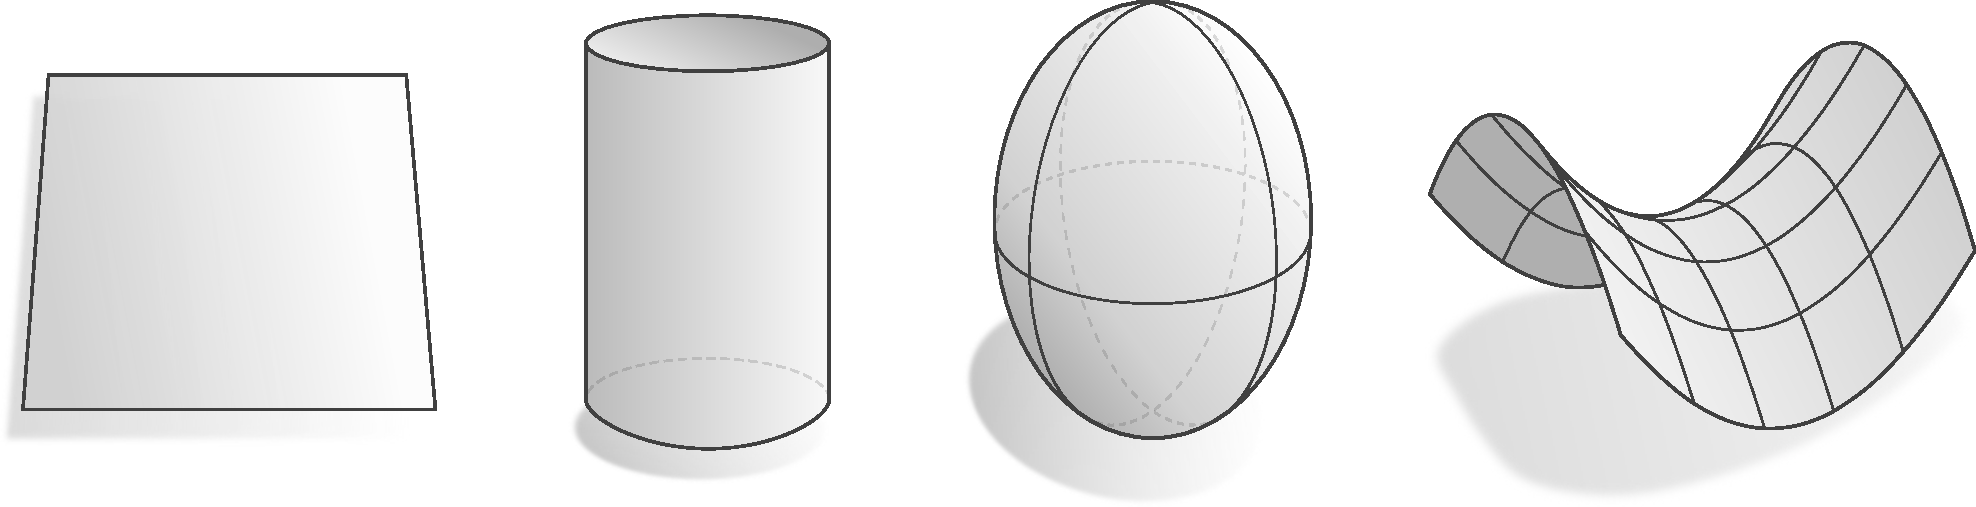
\includegraphics[width=1.\textwidth]{figures/curvature_surfaces.pdf}
    \caption{\small
        Embedded surfaces of qualitatively different extrinsic curvatures.
        \textit{Left:}
            The plane is characterized by vanishing principal and Gaussian curvatures
            $\kappa_{\max} = \kappa_{\min} = \kappa_{\textup{Gauss}} = 0$.
        \textit{Middle left:}
            A cylinder has one direction of positive curvature and one of vanishing curvature, i.e. 
            $\kappa_{\max} > 0$ and $\kappa_{\min} = 0$.
            Its Gaussian curvature $\kappa_{\textup{Gauss}} = 0$ is therefore zero as well.
            The plane and the cylinder are locally isometric, that is, their intrinsic geometry is locally indistinguishable.
            Note that the plane can be rolled up (developed) to form a cylinder -- the difference between the two is just the embedding into ambient space.
        \textit{Middle right:}
            An ellipsoid is characterized by its positive principal and Gaussian curvatures $\kappa_{\max} > 0$, $\kappa_{\min} > 0$ and $\kappa_{\textup{Gauss}} > 0$ at every point.
        \textit{Right:}
            The surface of a saddle bends in opposite directions, implying opposite signs of the principal curvatures $\kappa_{\max} > 0$ and $\kappa_{\min} < 0$.
            As a result, the Gaussian curvature $\kappa_{\textup{Gauss}} < 0$ is negative.
     }
    \label{fig:curvature_surfaces}
\end{figure}

Since $\GM$-convolutions depend only on the intrinsic geometry of a surface, the reader might wonder why we are discussing their extrinsic properties like principal curvatures.
The reason is that $\GM$-convolutions may nonetheless be informed about a surface's extrinsic geometry, for instance by encoding it in feature fields.
The extrinsic geometry may furthermore be used to heuristically align the frames of an $\{e\}$-structure and thus kernels.
For example, \citet{jin2018learning} and \citet{li2019crossAtlas} align the frames along the $z$-axis of the ambient space $\R^3$, while \citet{boscaini2016learning} and \citet{tatarchenko2018tangent} align the frames along the surface's dominant principal curvature direction.
Note that these heuristics are not always well defined:
for instance, the projection of the $z$-axis on a ``horizontal'' tangent space (in the ambient space) is zero,
and the dominant principal curvature direction might not be defined, as it is the case on the sphere.






















\subsubsection{Discretized geometry of surface meshes}
\label{sec:surfaces_geom_mesh}

In principle, it would be possible to describe $\GM$-convolutions on local surface parametrizations as described in the last section.
While this approach might be suitable for certain simple or symmetric geometries like ellipsoids, hyperboloids or tori, it seems impractical for more complex geometries.
In practice, surfaces come mostly discretized, for instance in form of triangle meshes, quad meshes, halfedge meshes, subdivision surfaces or point clouds.
Due to their widespread use -- both in general and specifically in the description of the surface $\GM$-convolutions that we review in the next two sections -- we will in the following focus primarily on triangle meshes.
Our goal for the remainder of the current section is therefore to take the quantities and definitions from the smooth theory and discuss their discrete counterparts on triangle meshes.
Unfortunately, these discrete analogues are usually not unique, such that a plethora of inequivalent definitions exists.%
\footnote{
    \citet{meyer2003discrete} describe this situation as follows:
    \emph{``Despite extensive use of triangle meshes in Computer Graphics, there is no consensus on the most appropriate way to estimate simple geometric attributes such as normal vectors and curvatures on discrete surfaces.''.}
    Similarly, \citet{craneDiscreteDifferentialGeometry2014} claims:
    \emph{``There is no one “right” way to discretize a given geometric quantity, but rather many different ways, each suited to a particular purpose.''}
}
We will in the following try to give a general idea about some of the most common approaches of discretizing the smooth geometry of surfaces in terms of triangle meshes.


\paragraph{Topology, geometry and embedding of triangle meshes:}
Triangle meshes $(\mathcal{V},\mathcal{F})$ are commonly encoded in terms of a set
\begin{align}
    \mathcal{V}\subseteq\N
\end{align}
of \emph{vertices} and a set
\begin{align}
    {\mathcal{F} \subseteq \big\{\mkern-2mu \{i,j,k\} \mkern2mu\big|\mkern2mu i\neq j\neq k \in\mathcal{V} \big\}}
\end{align}
of triangular \emph{faces},
satisfying that each vertex is contained in at least one of the faces.%
\footnote{
    Faces may alternatively be defined as ordered 3-tuples of vertices.
    The ordering of the vertices (or rather the equivalence classes of orderings under an even number of permutations) may then be used to encode the faces' orientations.
    We will instead encode face orientations as in our smooth theory by a choice of handedness of reference frames.
}
A set
\begin{align}
    \mathcal{E} = \big\{ \{i,j\} \,\big|\ i\neq j\in \{i',j',k'\} \textup{ for some } \{i',j',k'\} \in \mathcal{F} \big\}
\end{align}
of \emph{edges}, bounding the faces, follows immediately.
In practice, one is often given a set
\begin{align}
    P = \big\{ p_i \in \R^3 \,\big|\, i\in\mathcal{V} \big\}
\end{align}
of vertex positions, specifying an \emph{embedding} of the mesh in the ambient space~$\R^3$.
This embedding implies lengths
\begin{align}
    l_{\{i,j\}} = \lVert p_j-p_i \rVert
\end{align}
of edges $\{i,j\}$ and areas
\begin{align}
    \textup{A}_{\{i,j,k\}} = \frac{1}{2} \big\lVert {(p_j-p_i)} \times (p_k-p_i) \big\rVert
\end{align}
of faces $\{i,j,k\}$.


We are specifically interested in \emph{surface meshes}, which are required to satisfy additional conditions.
In order to formulate these conditions, note that the mesh elements $\{ i_0, \dots, i_n \}$
(where $n=0,1\ \text{or}\ 2$ for vertices, edges or faces)
imply $n$-\emph{simplices}, defined as the convex hulls
\begin{align}
    \operatorname{convex} \!\big(\{ i_0, \dots, i_n \}\big)\ :=\ 
    \Big\{ \sum\nolimits_{j=0}^n \alpha_j\mkern2mu p_{i_j} \,\Big|\, 
    \sum\nolimits_{j=0}^n \alpha_j = 1\,\ \textup{and}\,\ \alpha_j\geq0\,\ \forall\,j=0,\dots,n \Big\}
    \ \ \subset\ \R^3 \,.
\end{align}
The set that comprises all of these simplices (mesh elements) forms a \emph{pure $2$-simplicial complex}~\cite{desbrun2005DiscreteExteriorCalculus,craneDiscreteDifferentialGeometry2014}.
That the 2-simplicial complex is \emph{pure} means that each 0-simplex (vertex) and 1-simplex (edge) is a subset of at least one 2-simplex (face).
In other words, there are no disconnected vertices or edges in the mesh.
The \emph{underlying space}
\begin{align}
    \bigcup_{\{ i_0, \dots, i_n \} \in \mathcal{V} \cup \mathcal{E} \cup \mathcal{F}}
    \mkern-40mu
    \operatorname{convex} \!\big( \{ i_0, \dots, i_n \}\big)
    \ \ \overset{\textup{(pure)}}{=}\,
    \bigcup_{\{i,j,k\} \in \mathcal{F}}
    \mkern-10mu
    \operatorname{convex} \!\big( \{i,j,k\}\big)
    \ \ \ \subset\ \R^3
\end{align}
of the simplicial complex is defined as the union of all of its simplices, equipped with the usual topology as a subset of~$\R^3$.
A mesh is then said to be a surface mesh (manifold mesh) if the underlying space is a topological surface (manifold), optionally with boundary.
Intuitively, this requires
1) that each edge is adjacent to two faces (or one at boundaries) and
2) that the faces around each vertex form a topological disk (or a half-disk at boundaries).


Such defined surface meshes are discrete counterparts to \emph{embedded} Riemannian surfaces.
However, since $\GM$-convolutions are independent from the \emph{extrinsic} geometry of the underlying manifold, it is instructive to briefly discuss their \emph{intrinsic} geometry.
Take therefore the vertex, edge and face sets $\mathcal{V}$, $\mathcal{E}$ and $\mathcal{F}$, but discard the embedding locations $P$ of the vertices.
Together, these sets form an \emph{abstract 2-simplicial complex}
$\mathcal{V} \cup \mathcal{E} \cup \mathcal{F} \,,$
defined as a family of abstract simplices $\{i_0,\dots,i_n\}$ that is closed under taking subsets~\cite{craneDiscreteDifferentialGeometry2014}.
If this (now abstract) 2-simplicial complex is
1) pure and
2) such that the ``Star'' of every vertex (given by the simplices containing that vertex) form a combinatorial disk,
it forms an \emph{abstract simplicial surface} (which is exactly the case if the embedded mesh is a surface mesh).
Abstract simplicial surfaces can be viewed as combinatorial counterparts of topological manifolds.
They admit to compute topological invariants, for instance the Euler characteristic
\begin{align}
    \mathcal{X}_{\textup{Euler}} = |\mathcal{V}|-|\mathcal{E}|+|\mathcal{F}| \,.
\end{align}
As a topological invariant, the Euler characteristic agrees for any two homeomorphic spaces, in particular for a smooth manifold and any of its triangulations.
For instance, the icosahedron from Section~\ref{sec:spherical_CNNs_icosahedral} has $\mathcal{X}_{\textup{Euler}}^\textup{ico} = 12-30+20 = 2$, which agrees with $\mathcal{X}_{\textup{Euler}}^{S^2} = 2$ for the 2-sphere.


To arrive at an intrinsic description of a triangulated surface's \emph{geometry}, one assigns \emph{edge lengths} ${l_{ij} \in \R^+}$ to edges $\{i,j\} \in \mathcal{E}$.
For consistency, these lengths are required to satisfy the triangle inequality $l_{\{i,j\}} + l_{\{j,k\}} > l_{\{k,i\}}$ for any face $\{i,j,k\} \in \mathcal{F}$.
The edge lengths imply Euclidean metrics (distance functions) on the faces, and therefore a piecewise defined Euclidean metric on the whole surface.
It corresponds to a Riemannian metric (or first fundamental form) which is Euclidean away from vertices and ``cone-like'' (singular) on a small neighborhood around the vertices~\cite{Crane2020DiscreteConformalGeometry,desbrun2005DiscreteExteriorCalculus}.


In order to close the circle to our initial, extrinsic definition of triangle meshes, on needs to embed the mesh into ambient space~$\R^3$.
The necessary information on the extrinsic geometry is given by equipping the mesh with a \emph{second fundamental form}.
In the discrete setting, this form can be defined as a choice of dihedral angle (bending angle) between any two adjacent triangles, i.e. one angle per non-boundary edge of the mesh.
Provided that this data is chosen consistently%
\footnote{
    The discrete first and second fundamental forms are required to satisfy an integrability condition,
    similar to the Gauss's equation and the Mainardi-Codazzi equations in the smooth setting~\cite{wang2012surfaceReconstruction}.
},
it is possible to reconstruct the embedding, i.e. vertex positions~$P$, up to rigid motions in~$\E3$~\cite{lipman2005linear,wang2012surfaceReconstruction}.
While an embedding of the surface is not necessary for the intrinsic $\GM$-convolutions, all of the papers listed in rows (37-41) of Table~\ref{tab:network_instantiations} evaluate their models on embedded triangle meshes.



\paragraph{Tangent spaces and vector fields:}
To describe vector fields on meshes, and to equip the meshes with geometric structure like connections, it is necessary to define a notion of tangent spaces that are attached to them.
Multiple incompatible definitions, tailored towards the specific application in mind, occur in the literature.
Since vector fields are commonly sampled at discrete locations, the discrete tangent bundles are often only partially defined, for instance only on faces, edges or vertices.
We briefly review some of these definitions, a more detailed survey can be found in~\cite{deGoes2016VectorFieldProcessing}.


Since the faces (2-simplices) of an embedded mesh are flat, one can naturally define their tangent spaces as those two-dimensional subspaces of~$\R^3$ in which they are contained~\cite{craneTrivialConnectionsDiscrete2010,craneDiscreteDifferentialGeometry2014,wang2012surfaceReconstruction}.
Specifically, given a face $\{i,j,k\} \in \mathcal{F}$, one may define the tangent spaces $\TpM = \operatorname{span}(p_j-p_i,\, p_k-p_i) \subset \R^3$ for every $p\in \operatorname{convex}\!\big(\{i,j,k\}\big)$ as the \emph{linear span of any two edge vectors}.
The alignment of the tangent space in ambient space is often represented in terms of the face normal $n = (p_j-p_i) \times (p_k-p_i)$.
Discrete tangent (or feature) vector fields can in face based representations be defined as being face-wise constant, i.e. represented by a single tangent (or feature) vector per face.
Relative to a choice of reference frame on each of the faces, such tangent and feature vector fields are encoded by $2|\mathcal{F}|$ or $c|\mathcal{F}|$ vector coefficients, respectively.
Note that such vector fields do not extend to vertices or edges.
Due to their discontinuity, the notion of differential operators, acting on such fields, is quite limited~\cite{deGoes2016VectorFieldProcessing} (which is irrelevant for our specific application).
A linear interpolation scheme of face based vector fields was proposed in~\cite{li2006representing}.


As there is no natural normal direction at the vertices of a mesh, there are multiple common definitions of vertex tangent spaces.
\emph{Vertex normals} can for instance be defined as an area weighted average of the adjacent faces' normals~\cite{lipman2005linear,lai2009metric,deHaan2020meshCNNs}.
Besides area weighting, uniform weights or tip angle weights are sometimes used~\cite{craneDiscreteDifferentialGeometry2014}.
Another option is to define normal vectors via a mean curvature normal operator \cite{meyer2003discrete}.
The resulting normal agrees with normals derived via area gradients, but differs from those that are derived via volume gradients or sphere inscribed normals; see~\cite{craneDiscreteDifferentialGeometry2014}.


Alternatively, one can define vertex tangent spaces in an \emph{intrinsic} way, simply by defining them as two-dimensional vector spaces that are attached to the vertex.
Their relation to the mesh geometry in a local neighborhood around the vertex is hereby encoded by representing the one-ring neighborhood in the tangent planes.
The arguably most prominent of such approaches is based on a rescaling of the total angle
\begin{align}\label{eq:mesh_total_incident_angle}
    \Theta_i \,=\! \sum_{\{i,j,k\}\in\mathcal{F}} \theta_{\{i,j,k\}}^i \,,
\end{align}
which is summed from the tip angles
$\theta_{\{i,j,k\}}^i = \arccos \big\langle \frac{p_j-p_i}{\lVert p_j-p_i\rVert} \frac{p_k-p_i}{\lVert p_k-p_i\rVert} \big\rangle$
of all the triangles $\{i,j,k\}$ adjacent to vertex $i\in\mathcal{V}$.
If this angle is exactly $2\pi$, the local neighborhood around the vertex is intrinsically flat; see for instance the red or green neighborhood in Fig.~\ref{fig:ico_neighborhoods}.
An angle $\Theta_i < 2\pi$, as for the blue neighborhood, signals a positive discrete Gaussian curvature (properly defined below) $\kappa_{\textup{Gauss},i} = 2\pi - \Theta_i$, i.e. a cone-like neighborhood.
An angle $\Theta_i > 2\pi$ corresponds similarly to a saddle-like neighborhood with negative Gaussian curvature.
The approach followed in
\cite{polthier1998straightest,zhang2006vectorFieldDesign,Knoppel:2013:GOD,Sharp2019VectorHeatMethod,craneDiscreteDifferentialGeometry2014}
is then to \emph{flatten} the one-ring neighborhood out by isotropically \emph{rescaling polar angles} by a factor of $s_i = \frac{2\pi}{\Theta_i}$ to the total $s_i \Theta_i = 2\pi$ of a Euclidean (tangent) space.
A vector field can is in this setting be represented by one vector per vertex.
A choice of gauge, which are often aligned with one of the edges, allows then to encode tangent or feature vector fields in terms $2|\mathcal{V}|$ or $c|\mathcal{V}|$ coefficients, respectively.
\citet{zhang2006vectorFieldDesign} proposed to interpolate the vectors with a piecewise linear hat function weighting from the vertices to the faces.
The direction of the vectors is thereby determined by a usual Euclidean transport on the flattened tangent spaces.
As pointed out by~\citet{deGoes2016VectorFieldProcessing}, this interpolation is not continuous.
To resolve this issue, the same authors propose in \cite{liu2016discreteConnection} to define a smooth structure on the triangle mesh and to represent the one-ring neighborhoods in \emph{smooth charts}.
A smooth interpolation is then performed by transporting vectors via a smooth simplicial connection on the mesh, which is optimized to be as close as possible to the original embedding space induced Levi-Civita connection.
Note that both approaches are effectively flattening the geometry around the vertices, that is, they do not exactly operate on the triangle mesh.


Yet another approach, rooted in discrete exterior calculus~\cite{desbrun2005DiscreteExteriorCalculus,elcott2005building}, is to define tangent vectors $v = \omega^\sharp \in \TpM$ in terms of \emph{1-forms} $\omega \in \TspM$ by leveraging the (metric-dependent) musical isomorphism $\sharp^\eta: \TsM \to \TM$ (``index raising'').
Since simplicial 1-forms are naturally assigned to \emph{edges} (1-simplices), this leads to an vector fields which are parameterized in terms of one vector per edge and thus $2|\mathcal{E}|$ coefficients after choosing frames.
However, as argued by \citet{deGoes2016VectorFieldProcessing} a piecewise linear interpolation of the vectors over the faces will again lead to discontinuities.
It is furthermore not clear to us how this approach could be generalized to general associated vector bundles and thus feature fields.







Given any of the above constructions of tangent spaces, \emph{local reference frames} are readily defined as 2-tuples of linearly independent tangent vectors.
A common choice is thereby to align the first frame axis with one of the adjacent edges of the current simplex (mesh element).
Specifically for the case of orthonormal, right-handed frames, i.e. whenever $G\leq\SO2$, a choice of (oriented) edge determines a frame completely.
Tangent vectors are then often represented in polar coordinates, with the angle measured relative to the reference edge.
If the tangent spaces are modeled extrinsically, that is, as two-dimensional subspaces of the ambient space $\R^3$, it is most common to represent the frames explicitly as a 2-tuple of vectors in $\TpM \subset \R^3$.
The definitions of frames and gauges are then fully equivalent to those in 
Eqs.~\eqref{eq:embedding_gauge_map_orthonormal_frame} and~\eqref{eq:embedding_space_R3_frame}
in Section~\ref{sec:sphere_geometry}.

$G$-structures are, as usual, defined as bundles of frames, which are in each tangent space related through $G$-valued gauge transformations.
In the computer graphics community, there is a particular interest in \emph{$N$-direction fields} (or unit $N$-RoSy fields), which are there defined as a collection of $N$ unit vector fields, such that the $N$ vectors in each tangent space are spaced by an angle of~$2\pi/N$.
Since any unit vector implies on an oriented manifold a corresponding right-handed, orthonormal frame, $N$-direction fields are seen to be equivalent to $\CN$-structures.
An example is the $\C6$-structure on the icosahedron in Fig.~\ref{fig:G_structure_ico_3}, which effectively assigns $6$ unit directions to each point, except for the poles, where it has singularities of index $\frac{1}{6}$ (or angle $\frac{2\pi}{6}$).
The interactive design of smooth direction fields, with user defined singularities amongst other constraints, is an active field of research in the computer graphics community
\cite{li2006representing,ray2008nSymmDirectionField,lai2009metric,craneTrivialConnectionsDiscrete2010,Knoppel:2013:GOD,liu2016discreteConnection,Sharp2019VectorHeatMethod}.
Some of the surface $\GM$-convolutions that we review in the following section use such algorithms to compute a $\CN$-structure~\cite{huang2019texturenet,Yang2020parallelFrameCNN}.



\paragraph{Riemannian metric and isometries:}
Having a mesh equipped with tangent spaces, one can define a \emph{Riemannian metric} on it.
The most common case that of isometrically embedded meshes with tangent spaces modeled as two-dimensional subspaces of the ambient space~$\R^3$.
As described before in Eqs.~\eqref{eq:spherical_embedding_metric_explicit} and~\eqref{eq:surface_embedding_metric}, the metric is then induced by restricting the standard Euclidean inner product $\langle\cdot,\cdot\rangle_{\R^3}$ of the embedding space to the tangent spaces.

If the tangent spaces are modeled intrinsically, a metric can be fixed by choosing an $\O{d}$-structure, i.e. reference frames that are \emph{defined} to be orthonormal.
Somewhat less tautological, if one is given edge lengths~$l_{\{i,j\}}$, and therefore a piecewise defined Euclidean distance function on the surface as discussed above, the choice of $\O{d}$-structure is required to be compatible with these lengths.
Specifically, the logarithmic map should result in tangent vectors of (Riemannian) norm $|\log_p(q)| = \mathscr{d}$ if the points $p$ and~$q$ are separated by a Euclidean distance $\mathscr{d} \in \R^+$.
Note that this statement requires a consistent definition of Levi-Civita connection on the mesh, which we discuss further below.


\emph{Isometries} are intrinsically defined as usual, that is, as those mappings of the mesh to itself, which preserve the metric.
Extrinsically, the isometry group is comprised of those isometries $\phi \in \E2$ of the embedding space, which leave the mesh invariant.
Most of the papers in
rows (37-41)
of Table~\ref{tab:network_instantiations}
consider datasets whose meshes have a trivial isometry group.
However, local neighborhoods of the meshes are often nonetheless isometric (or approximately isometric) to each other, which was exemplified in Fig.~\ref{fig:suzanne_local_isometry}.
As discussed in Section~\ref{sec:isometry_groups}, the isometry equivariance of $\GM$-convolutions will still hold locally if the kernels' field of view is sufficiently small.







\paragraph{Connections, transporters and geodesics on triangle meshes:}
The last ingredient that we need to implement $\GM$-convolutions on meshes is the transporter pullback $\Expsp$ of feature fields, Eq.~\eqref{eq:transporter_pullback_in_coords}.
We are therefore required to know how to
1) parallel transport feature vectors over meshes and
2) compute geodesics on meshes, specifically the exponential map or, depending on the implementation, the logarithmic map.
All of these mappings depend ultimately on a choice of \emph{connection} on the mesh.
In the smooth setting, a connection is essentially a collection of infinitesimal transporters between adjacent tangent spaces.
One defines discretized connections on meshes therefore usually as transporters between adjacent mesh elements.
The particular choice of tangent bundle discretization, options of which were discussed above, influences the particular definition of connection.
In the following, we review some discretizations of connections found in the literature and explain how they can be used to compute transporters and geodesics.


The simplest case to consider is the transport or connection between two adjacent faces.
Recall that the Levi-Civita transport on a flat plane is defined as shifting a vector such that it stays parallel in the usual Euclidean sense; see Fig.~\ref{fig:transport_flat}.
As connections are inherently intrinsic, they do not depend on the particular embedding of this plane into ambient space, which tells us how to transport on any developable surface.
It tells us in particular how to transport between two adjacent triangles, since they can be unfolded (developed) into a plane as visualized in Fig.~\ref{fig:transport_mesh}.
The Levi-Civita connection between faces can therefore be thought of as
1)~flattening the faces
2)~transporting the vector as usual on the plane and
3)~folding the faces back to their original embedding~\cite{craneTrivialConnectionsDiscrete2010,mitchell1987discrete,craneDiscreteDifferentialGeometry2014}.
The resulting transporter
$\mathcal{P}_{\mkern-2mu\overset{}{\protect\scalebox{.62}{$\!T\!M$},\protect\scalebox{.68}{$\{i,j,k\mkern-1mu\}\!\to\!\{i,j,l\}$}}}$
between the faces $\{i,j,k\}$ and $\{i,j,l\}$ can optionally be expressed in terms of a group element
$g^{A\widetilde{A}}_{\protect\scalebox{.68}{$\{i,j,k\mkern-1mu\}\!\to\!\{i,j,l\}$}}$ in~$\GL{2}$.
Since the Levi-Civita connection is a metric connection, it results for the specific case of orthonormal frames in group elements in~$\O2$, and for oriented orthonormal frames in $\SO2$-elements or rotation angles.

\begin{figure}
    \centering
    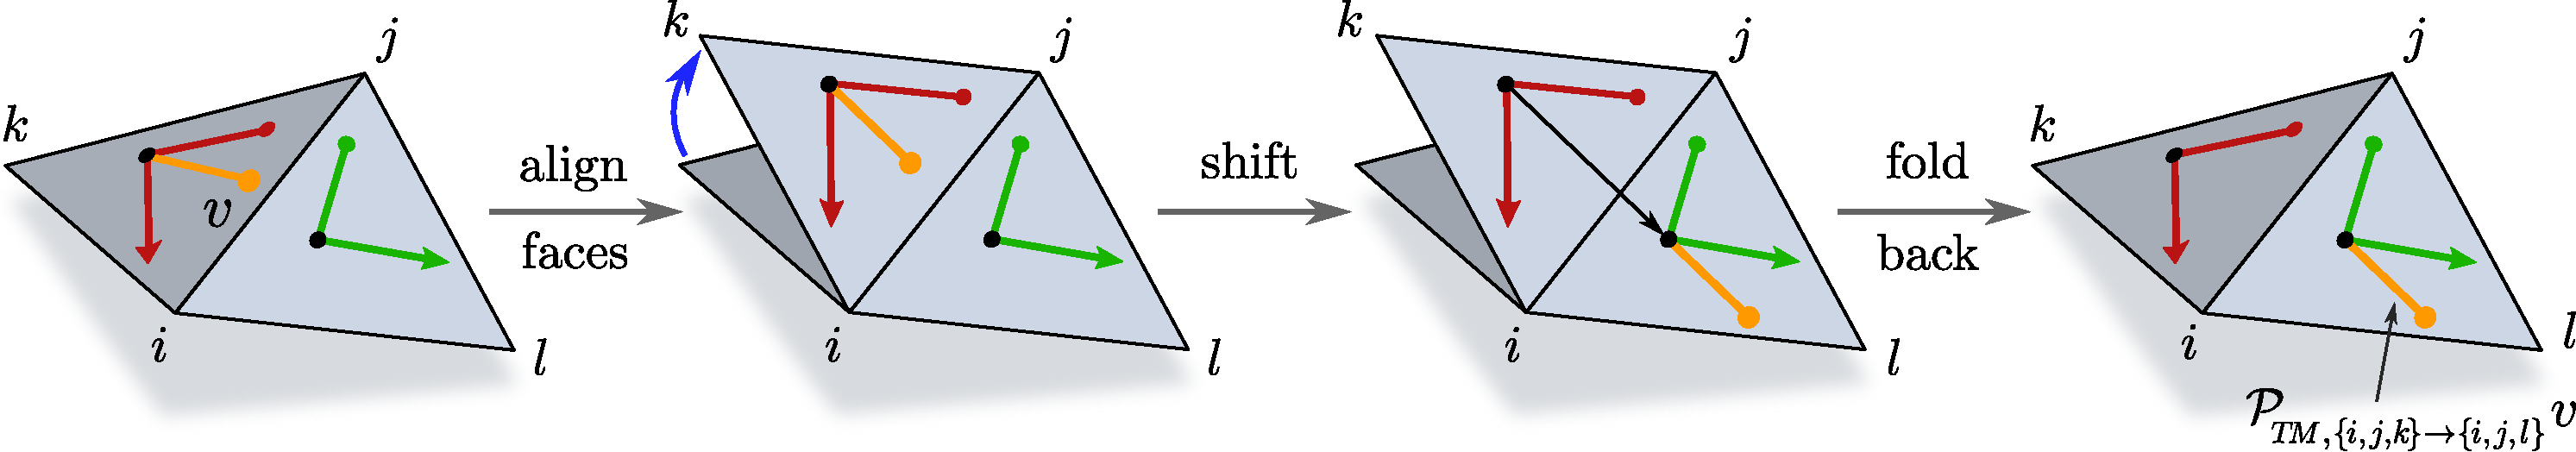
\includegraphics[width=1.\textwidth]{figures/transport_mesh.pdf}
    \caption{\small
        Parallel transport between mesh faces.
        The local geometry of two adjacent faces is developable, that is, it is intrinsically flat and can be unfolded into a plane.
        The Levi-Civita transport between the faces is therefore given by shifting a vector over the unfolded faces, followed by bending the faces back to their original embedding.
        This parallel transport between adjacent faces can be viewed as the discrete analog of the continuous Levi-Civita connection in the smooth setting~\cite{craneTrivialConnectionsDiscrete2010}.
        Given any choice of reference frames, the transport
        $\mathcal{P}_{\mkern-2mu\overset{}{\protect\scalebox{.62}{$\!T\!M$},\protect\scalebox{.68}{$\{i,j,k\mkern-1mu\}\!\to\!\{i,j,l\}$}}}$
        is represented by a group element
        $g^{A\widetilde{A}}_{\protect\scalebox{.68}{$\{i,j,k\mkern-1mu\}\!\to\!\{i,j,l\}$}} \in \GL{2}$ (or $\SO2$ when considering right-handed, orthonormal frames).
        More general connections apply an additional linear transformation to the coordinate free vector when transitioning between the faces.
        Alternative definitions of discrete connections, for instance for the transport between vertices along edges, are discussed in the main text.
    }
    \label{fig:transport_mesh}
\end{figure}


As proposed by \citet{craneTrivialConnectionsDiscrete2010}, it is possible to generalize this construction beyond Levi-Civita connections:
instead of merely shifting vectors between the flattened faces, more general connections apply an additional linear transformation, for instance an additional rotation.
While this additional transformation will be reflected by a corresponding transformation of the transporter's coordinate expression
$g^{A\widetilde{A}}_{\protect\scalebox{.68}{$\{i,j,k\mkern-1mu\}\!\to\!\{i,j,l\}$}}$,
it is conceptually independent from it and can be defined in a purely coordinate free setting.
The authors use this idea to construct smooth trivial connections, which are defined by having a transport of zero holonomy around any possible loop, and which are optimized to be as smooth as possible, except for at some singularities, which are topologically enforced~\cite{craneTrivialConnectionsDiscrete2010}.
They consider furthermore connections which apply (coordinate free) rotations by $\frac{2\pi}{N}$ and can be used to construct $N$-direction fields, corresponding to $\CN$-structures.
In our applications, we will \emph{always} consider Levi-Civita connections to compute geodesics.
The models reviewed in the following Section~\ref{sec:so2_surface_conv} assume a structure group $G=\SO2$ on oriented meshes and utilize Levi-Civita transporters for feature vectors.
In contrast, the models in Section~\ref{sec:e_surface_conv} assume a trivial structure group $G=\{e\}$ and therefore allow only for $\{e\}$-structure compatible trivial connections.
They transport features such that their coefficient vectors relative to the $\{e\}$-structure frames remain invariant, i.e. merely copy their numerical values.


Given embedded tangent spaces $\TpM \subset \R^3$ at other mesh elements like vertices or edges, this approach is naturally generalized to transitions between arbitrary mesh elements~\cite{deHaan2020meshCNNs}:
instead of aligning the faces, one could e.g. align the vertex tangent space with the adjacent face before shifting the vector.
Geometrically, this operation can be thought of as the transport over a mesh whose vertices and edges are cut off in an infinitesimal neighborhood, an are replaced with a polygonal face.


An alternative definition of discrete connections is given in \cite{Knoppel:2013:GOD} and \cite{Sharp2019VectorHeatMethod}.
The authors of both papers model tangent spaces only at the vertices, where they are defined in terms of the rescaling of the total incident angle, Eq.~\eqref{eq:mesh_total_incident_angle}, to $2\pi$, as discussed above.
A connection on the mesh is then given by transporters over all edges $\{i,j\} \in\mathcal{E}$, which link the adjacent vertices' tangent spaces.
Since the geometric notion of unfolding triangles is hereby missing, the edge transporters are encoded via group elements relative to a source and reference frame.
Specifically for the Levi-Civita connection, and orthonormal, right-handed reference frames, these group elements lie in~$\SO2$.
The utility of this construction for the direct transport along arbitrary paths over the manifold is unclear, however, it is useful to solve PDEs that depend on the covariant derivative.
\citet{Sharp2019VectorHeatMethod} showed that a solution of the vector heat equation allows nonetheless to use such connections to (indirectly) compute the parallel transport between arbitrary points on a mesh.
\citet{liu2016discreteConnection} propose yet another construction, namely smooth simplicial connections between and within all mesh elements.
They discuss furthermore how such connections can be optimized to be as close to the (non-smooth) Levi-Civita connection as possible.


A given connection determines the \emph{parallel transport} along a path.
In the smooth setting, where connections are infinitesimal transporters, the finite transport is computed by integrating the connection along the path.
In the discrete setting, the transport is accordingly given by composing the individual transformations that constitute the connection between the mesh elements that are crossed by the path.
For the Levi-Civita connection, this process corresponds to a flattening of all the mesh elements along the path, followed by shifting the vector over it; see Fig.~7 in~\cite{lai2009metric}.
The vector heat equation based method by \citet{Sharp2019VectorHeatMethod} computes the transport of vectors specifically along geodesics.
Since it solves for the transport from a source location to \emph{any} other location on the manifold simultaneously, this approach can be more efficient than integrating the transport for every single path individually.


The \emph{curvature of a connection} is in the smooth setting defined as the holonomy of its transport around an infinitesimally small disk.
The curvature at a vertex is in the discrete setting similarly defined as the holonomy of the transport around this vertex.
For the Levi-Civita connection, this is just the Gaussian curvature, which is given by the angle defect
\begin{align}
    \kappa_{\textup{Gauss},i} \,=\, \delta_i \,=\, 2\pi - \Theta_i \,,
\end{align}
where $\Theta_i$ is the total tip angle from Eq.~\eqref{eq:mesh_total_incident_angle}.
We refer again to the icosahedron as example, which has vanishing curvature everywhere, except for its original twelve vertices, where the angle defect (curvature) equals~$\frac{2\pi}{6}$.
Trivial connections have by construction zero curvature.


Lastly, we need to discuss \emph{geodesics}.
In the smooth setting, geodesics are defined as \emph{straightest paths}, which is formalized by the statement that the covariant derivatives of their tangent vectors along the curve vanish, that is, $\nabla_{\dot{\gamma}} \dot{\gamma} = 0$.
This is equivalent to the requirement that the transport of a tangent vector $\dot{\gamma}(t_0)$ along the geodesic remains tangent to it, i.e.
$\mathcal{P}_{\mkern-2mu\overset{}{\protect\scalebox{.6}{$\!T\!M$}, \gamma(t_1) \leftarrow \gamma(t_0)}}
 \dot{\gamma}(t_0) = \dot{\gamma}(t_1)$
for arbitrary $t_0$ and $t_1$.
Furthermore, the \emph{shortest path} between any two points on a connected manifold is given by a geodesic.
As pointed out by \citet{polthier1998straightest}, this equivalence of shortest and straightest paths does not longer hold on meshes, such that one needs to distinguish between the two concepts.


Recall that the \emph{exponential map} $\exp_p: \TpM \to M$ is defined as mapping vectors $v$ to that point which is reached when walking for a distance of $\lVert v\rVert$ from $p$ along the (unit speed) geodesic in direction of $v$.
This concept is readily generalized to meshes, where one follows the \emph{straightest geodesic} in the direction of $v$ for distance $\lVert v\rVert$.
As in the smooth setting, one may define such straightest geodesics on meshes as those curves that keep their tangent vector parallel to the curve.
This property is naturally satisfied on the planar faces (or along edges), such that the resulting geodesic is \emph{piecewise linear}, with the only nontrivial points being those where the geodesics transitions between adjacent mesh elements.
The outgoing direction of the geodesic after such a transition is thereby determined by the connection, i.e. by the transport of the incoming tangent direction to the next mesh element.
If one considers the Levi-Civita connection, which we always do to compute geodesics, this results in an ordinary straight line after unfolding the mesh elements into a plane.
To implement the discrete exponential map, it is sufficient to trace out such a straightest geodesic until reaching the distance $\lVert v\rVert$.


\emph{Logarithmic maps} $\log_p: M \to \TM$, on the other hand, can be thought of as computing the \emph{shortest geodesics} between points $p$ and $q$.
They return that vector $\log_p(q)$ in $\TpM$ which is tangent to this geodesic at $p$ and whose norm equals the geodesic distance between the points.
A prominent way of computing geodesic distances from a source point (or set) $p$ is to solve the eikonal equation
\begin{align}\label{eq:eikonal_equation}
    |\nabla \tau| = 1
    \quad\textup{subject to}\quad
    \tau(p) = 0 \,,
\end{align}
where $\nabla$ denotes the covariant derivative.
The first part of this PDE enforces the natural requirement that the gradient of the distance function should be one, while the second part fixes the distance at the source to zero.
A Fast Marching algorithm, which solves the eikonal equation on triangle meshes, was proposed by \citet{kimmel1998computingGeodesics}.
Given the distance function $\tau$, the geodesic $\gamma$ between $p$ and any other point $q$ can be traced back by following the distance gradient starting from $q$, i.e. by solving the ODE
\begin{align}
    \dot{\gamma} = -\nabla \tau \,.
\end{align}
With this information, we know that $\lVert\log_p(q)\rVert = \tau(q)$, with the direction of $\log_p(q)$ given by geodesic path at $p$.
The solution by \citet{mitchell1987discrete} generalizes the Dijkstra algorithm for computing distances along edges of a graph to a continuous version, which can cross faces and therefore operate on meshes.
It computes a distance function by propagating a wavefront starting from~$p$.
The heat method by \citet{Crane2017HeatMethodDistance} computes geodesic distances by exploiting Varadhan’s formula, which establishes a connection to the heat kernel.
Their algorithm is essentially solving the heat equation $\dot{u} = \Delta u$ with initial condition $u_0 = \delta(p)$, i.e. it diffuses a ``heat spike'' from the source point $p$.
For short diffusion times, the gradient $\nabla u$ points exactly in the opposite direction of the geodesic distances' gradient.
Since it is known that the geodesic distance gradient has unit magnitude (Eq.~\eqref{eq:eikonal_equation}), one can compute the distance field from this information.
The method is substantially faster than previous algorithms.
\citet{Sharp2019VectorHeatMethod} generalize this method to the vector heat equation, which allows to diffuse vector-valued quantities instead of scalar heat.
The algorithm can be used to transport vectors from a source point (or set) over the whole manifold, but it also suitable for solving with high accuracy for logarithmic maps.
